
\RequirePackage{fix-cm}
\documentclass[border=2pt]{standalone}

\usepackage{amsmath,amssymb,bm}
\usepackage{xcolor}
\usepackage{tikz}
\usetikzlibrary{arrows.meta,calc}

% Publication-oriented, colorblind-safe palette.
\definecolor{AdamRed}{HTML}{2CA02C}
\definecolor{Ink}{HTML}{1F1F1F}
\definecolor{ReachGray}{HTML}{767676}
\definecolor{FrameGray}{HTML}{D9DDE2}
\definecolor{CanvasLabel}{HTML}{62676D}

% Manuscript notation used by the user's revised labels.
\newcommand{\thetab}{\bm{\theta}}
\newcommand{\x}{\mathbf{x}}
\newcommand{\kb}{\mathbf{k}}

\begin{document}

% Presentation mode: research.
% Communication job: initialization-dependent reachability of the entire
% hypersurface, followed by the local KKT/normal relation at one limit point.
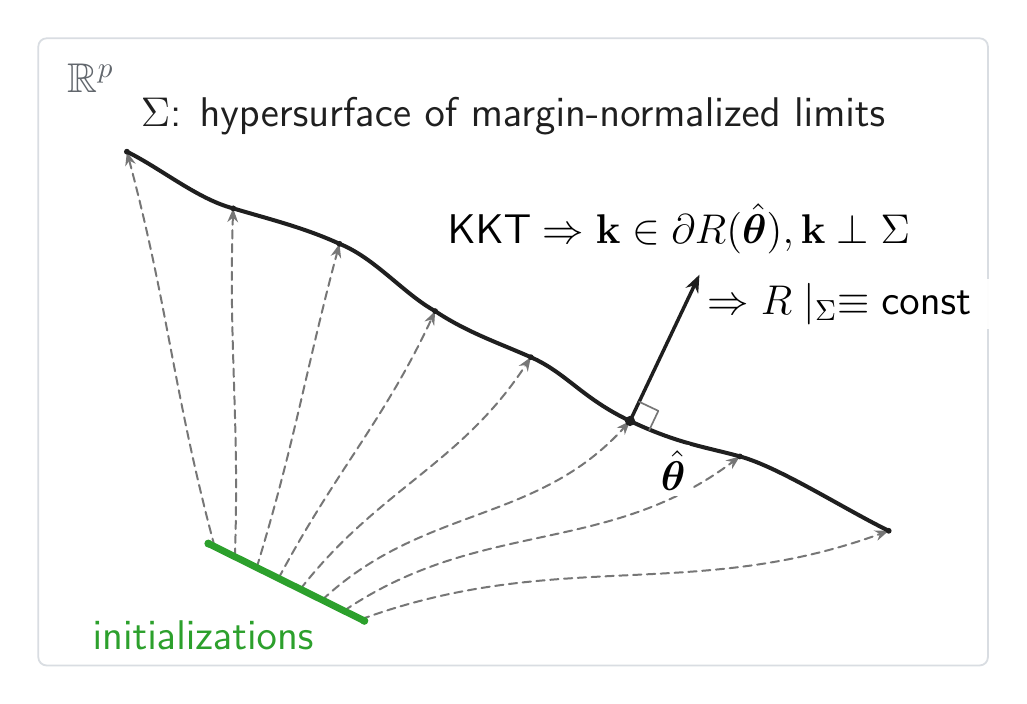
\begin{tikzpicture}[
  x=0.90cm,
  y=0.90cm,
  font=\sffamily\fontsize{15}{12}\selectfont,
  line cap=round,
  line join=round,
  surface/.style={draw=Ink, line width=1.45pt},
  initialization/.style={draw=AdamRed, line width=2.5pt},
  reach/.style={
    draw=ReachGray,
    densely dashed,
    line width=0.72pt,
    -{Stealth[length=1.75mm,width=1.35mm]}
  },
  normal/.style={
    draw=Ink,
    line width=1.25pt,
    -{Stealth[length=2.25mm,width=1.75mm]}
  },
  directlabel/.style={inner sep=1.5pt},
  annotation/.style={inner sep=1.5pt}
]

% --------------------------------------------------------------------------
% Ambient parameter space
% --------------------------------------------------------------------------
\path[use as bounding box] (0.15,0.15) rectangle (13.85,9.30);
\fill[white] (0.15,0.15) rectangle (13.85,9.30);
\draw[draw=FrameGray, line width=0.65pt, rounded corners=3pt]
  (0.30,0.30) rectangle (13.70,9.15);

\node[
  directlabel,
  text=CanvasLabel,
  anchor=north west
] at (0.65,8.85) {$\mathbb{R}^{p}$};

% --------------------------------------------------------------------------
% Initialization family in the lower-left corner
% --------------------------------------------------------------------------
\coordinate (init-start) at (2.70,2.02);
\coordinate (init-end)   at (4.90,0.93);

\coordinate (Ione)   at ($(init-start)!0.04!(init-end)$);
\coordinate (Itwo)   at ($(init-start)!0.17!(init-end)$);
\coordinate (Ithree) at ($(init-start)!0.31!(init-end)$);
\coordinate (Ifour)  at ($(init-start)!0.45!(init-end)$);
\coordinate (Ifive)  at ($(init-start)!0.59!(init-end)$);
\coordinate (Isix)   at ($(init-start)!0.73!(init-end)$);
\coordinate (Iseven) at ($(init-start)!0.87!(init-end)$);
\coordinate (Ieight) at ($(init-start)!0.98!(init-end)$);

% --------------------------------------------------------------------------
% Representative targets spanning the visible hypersurface
% --------------------------------------------------------------------------
\coordinate (Tone)   at (1.55,7.55);
\coordinate (Ttwo)   at (3.05,6.75);
\coordinate (Tthree) at (4.55,6.25);
\coordinate (Tfour)  at (5.90,5.30);
\coordinate (Tfive)  at (7.25,4.65);
\coordinate (hat-theta) at (8.65,3.75);
\coordinate (Tseven) at (10.20,3.25);
\coordinate (Teight) at (12.30,2.20);

% Dashed Adam trajectories. Their targets span the full displayed portion of
% Sigma_{B,C}; the curves are qualitative and do not encode training time.
\draw[reach] (Ione)   to[out=105,in=-75]  (Tone);
\draw[reach] (Itwo)   to[out=88,in=-92]   (Ttwo);
\draw[reach] (Ithree) to[out=73,in=-105]  (Tthree);
\draw[reach] (Ifour)  to[out=62,in=-115]  (Tfour);
\draw[reach] (Ifive)  to[out=52,in=-123]  (Tfive);
\draw[reach] (Isix)   to[out=43,in=-132]  (hat-theta);
\draw[reach] (Iseven) to[out=34,in=-143]  (Tseven);
\draw[reach] (Ieight) to[out=20,in=-160]  (Teight);

% Slightly nonlinear/squiggly rendering of the hypersurface. Explicit Bezier
% controls make the local tangent at hat-theta exactly parallel to
% (2.95,-1.40), the secant from Tfive to Tseven.
\draw[surface]
  (Tone)
  .. controls (2.02,7.32) and (2.55,6.88) .. (Ttwo)
  .. controls (3.55,6.60) and (4.05,6.48) .. (Tthree)
  .. controls (5.05,6.05) and (5.45,5.55) .. (Tfour)
  .. controls (6.35,5.00) and (6.80,4.85) .. (Tfive)
  .. controls (7.75,4.43) and (7.9715,4.072) .. (hat-theta)
  .. controls (9.3285,3.428) and (9.73,3.38) .. (Tseven)
  .. controls (10.75,3.10) and (11.65,2.52) .. (Teight);

% Small target marks reinforce that varying initialization covers the visible
% hypersurface rather than selecting a single preferred limit.
\foreach \target in {Tone,Ttwo,Tthree,Tfour,Tfive,Tseven,Teight}{
  \fill[Ink] (\target) circle (1.05pt);
}

\node[
  directlabel,
  anchor=south west,
  text=Ink,
  fill=white,
  fill opacity=0.92,
  text opacity=1
] at (1.68,7.72) 
% {Margin-normalized limits: $\Sigma = \{\thetab: f(\x_1; \thetab)=1\}$}
{$\Sigma$: hypersurface of margin-normalized limits }
;

\draw[initialization] (init-start) -- (init-end);
\fill[AdamRed] (init-start) circle (1.45pt);
\fill[AdamRed] (init-end) circle (1.45pt);

\node[
  directlabel,
  text=AdamRed,
  anchor=north west
] at (1.,1.) {initializations};

% --------------------------------------------------------------------------
% A normal at a selected limiting point
% --------------------------------------------------------------------------
\fill[Ink] (hat-theta) circle (1.85pt);
\node[
  annotation,
  anchor=north west,
  fill=white,
  rounded corners=1.2pt,
  inner sep=2.0pt,
  text opacity=1
] at (9.00,3.42) {$\hat{\boldsymbol\theta}$};

% At hat-theta the tangent is parallel to (2.95,-1.40). The displayed normal
% uses 0.70(1.40,2.95)=(0.98,2.065), whose dot product with the tangent is 0.
\coordinate (normal-end) at (9.63,5.815);
\draw[normal] (hat-theta) -- (normal-end);

% Right-angle marker between the local tangent and the displayed normal.
\begin{scope}[shift={(hat-theta)}, rotate=-25.385]
  \draw[draw=ReachGray, line width=0.60pt]
    (0.30,0) -- (0.30,0.30) -- (0,0.30);
\end{scope}

\node[
  directlabel,
  anchor=south,
  align=left,
  fill=white,
  fill opacity=0.95,
  text opacity=1
] at (9.63,6.04) {%
  $\begin{aligned}
    % \mathbf{k} &\in \partial R(\hat{\boldsymbol\theta}),\\[-1pt]
    % \mathbf{k} &\propto \mathbf{h}
    %   \in \partial\, y f(\mathbf{x}_1;\hat{\boldsymbol\theta})
    %   \Rightarrow \kb \perp \Sigma
    \text{KKT} \Rightarrow\mathbf{k} \in \partial R(\hat \thetab) & , \mathbf k \perp \Sigma
  \end{aligned}$
};


\node[
  directlabel,
  anchor=south,
  align=left,
  fill=white,
  fill opacity=0.95,
  text opacity=1
] at (11.7,5.04) {%
  $\begin{aligned}
    % \mathbf{k} &\in \partial R(\hat{\boldsymbol\theta}),\\[-1pt]
    % \mathbf{k} &\propto \mathbf{h}
    %   \in \partial\, y f(\mathbf{x}_1;\hat{\boldsymbol\theta})
    %   \Rightarrow \kb \perp \Sigma
    \Rightarrow R \mid_{\Sigma} \equiv  \text{const} 
  \end{aligned}$
};

% \node[
%   directlabel,
%   text=Ink,
%   anchor=north,
%   align=center,
%   fill=white,
%   fill opacity=0.94,
%   text opacity=1
% ] at (11.40,1.55) {margin-normalized\\limits hypersurface $\Sigma$};

\end{tikzpicture}

\end{document}
